\chapter{The Error-State Kalman Filter}
\label{ch:eskf}

\begin{objectives}
\begin{itemize}
  \item Understand the three-way split into true, nominal and error state, and why it is the right way to filter on a manifold.
  \item Derive the linearized error dynamics with a mechanical recipe.
  \item Define measurement residuals and Jacobians on the manifold with the correct sign convention.
  \item Derive the injection and reset steps, including the reset Jacobian $G$.
  \item Assemble the complete error-state Kalman filter loop, and follow it through a complete attitude-estimation example.
\end{itemize}
\end{objectives}

% ==============================================================================
\section{Filtering on a manifold}

The EKF of \cref{ch:nonlinear} assumes the state lives in $\R^n$, so that $\hat x + Kr$ makes sense. For VIO, the state contains a rotation, which does
not live in a vector space (\cref{ch:lie}). Three quantities must therefore be distinguished.

\begin{definition}[True, nominal and error state]
\index{error state}\index{nominal state}
\begin{itemize}
  \item The \textbf{true state} $x$ is the unknown physical state, a point on the state manifold $\mathcal{M}$.
  \item The \textbf{nominal state} $\hat x \in \mathcal{M}$ is the current best estimate, propagated with the full nonlinear model and no noise.
  \item The \textbf{error state} $\delta x = x \bminus \hat x \in \R^{n}$ is the small, minimal-dimension difference, defined with the operators of
        \cref{sec:boxplus}.
\end{itemize}
The filter's Gaussian belief is over the error state: $\delta x \sim \N(\delta\hat x, P)$, so that $x = \hat x \bplus \delta x$.
\end{definition}

For the IMU state this means 16 nominal numbers (quaternion included) but a 15-dimensional error and a $15\times15$ covariance, with no redundant
directions and no constraints. The Kalman filter operates only on the error state, which is a vector, so all of \cref{ch:kf} applies to it. This
design is called the \term{error-state Kalman filter} (ESKF), or \emph{indirect} Kalman filter. In aerospace the same idea for attitude is the
\emph{multiplicative} EKF.

\begin{keyidea}[why the error state]
\begin{itemize}
  \item \textbf{Minimal and unconstrained.} The error has exactly as many components as degrees of freedom, so its covariance is non-singular and
        needs no constraint handling.
  \item \textbf{Always near the origin.} After every update the error is reset to zero, so it never approaches the singularities of
        three-parameter rotations, and the small-angle approximations used to derive its dynamics remain valid.
  \item \textbf{Nearly linear.} The large, fast, nonlinear motion is carried by the nominal state, which is integrated exactly. The error evolves
        slowly and is small, so its dynamics are almost linear and linearization is accurate (\cref{ch:nonlinear}).
  \item \textbf{Slow.} Error dynamics are governed by sensor errors, not by vehicle motion, so the covariance could even be propagated at a lower rate
        than the nominal state if computation were scarce.
\end{itemize}
\end{keyidea}

% ==============================================================================
\section{The ESKF cycle}

\begin{figure}[t]
\centering
\begin{tikzpicture}[node distance=14mm and 30mm]
  \node[block, minimum width=40mm] (nom) {\textbf{1. Nominal propagation}\\ $\hat x \gets f(\hat x, u)$, noise-free, nonlinear};
  \node[block, minimum width=40mm, right=of nom] (cov) {\textbf{2. Covariance propagation}\\ $P \gets \Phi P\Phi\T + Q_d$};
  \node[block, minimum width=40mm, below=of cov] (upd) {\textbf{3. Update}\\ $r = z\bminus h(\hat x)$, \ $\delta\hat x = Kr$\\ $P \gets$ Joseph form};
  \node[block, minimum width=40mm, below=of nom] (inj) {\textbf{4. Inject and reset}\\ $\hat x \gets \hat x\bplus\delta\hat x$, \ $\delta\hat x \gets 0$\\ $P \gets GPG\T$};
  \draw[->, thick] (nom) -- node[note, above]{every IMU} node[note, below]{sample} (cov);
  \draw[->, thick] (cov) -- node[note, right, align=left]{measurement\\arrives} (upd);
  \draw[->, thick] (upd) -- (inj);
  \draw[->, thick] (inj) -- (nom);
  \draw[->, thick, dashed] (cov.north) to[out=135, in=45] node[note, above]{no measurement: next IMU sample} (nom.north);
\end{tikzpicture}
\caption{The error-state Kalman filter cycle. The error-state mean is zero throughout propagation, so only the covariance is propagated in step 2. It
becomes non-zero in step 3 and is transferred to the nominal state and zeroed in step 4.}
\label{fig:eskf-cycle}
\end{figure}

\Cref{fig:eskf-cycle} shows the four steps.
\begin{enumerate}
  \item \textbf{Nominal propagation.} At each IMU sample, integrate the nonlinear kinematics with the measured inputs, ignoring noise
        (\cref{ch:strapdown}).
  \item \textbf{Error covariance propagation.} Propagate $P$ with the linearized error dynamics (\cref{ch:errordyn}).
  \item \textbf{Update.} When a measurement arrives, compute the residual and its Jacobian on the manifold, and compute the Kalman estimate of the
        error, $\delta\hat x = Kr$, and the posterior covariance.
  \item \textbf{Injection and reset.} Move the estimated error into the nominal state with $\bplus$, set the error mean back to zero, and correct the
        covariance for the change of reference point.
\end{enumerate}

\begin{proposition}[The error mean needs no propagation]
If $\delta\hat x = 0$ after a reset, and the error obeys linear dynamics $\dot{\delta x} = F_c\delta x + G_cw$ with zero-mean noise, then $\E[\delta x] = 0$ until the
next update.
\end{proposition}
\begin{proof}
The mean obeys $\frac{\dd}{\dd t}\E[\delta x] = F_c\,\E[\delta x]$ (\cref{prop:lyapunov}) with initial value zero, whose unique solution is zero.
\end{proof}

This is why step 2 propagates only the covariance: all the knowledge of the error state's mean has been transferred into the nominal state.

% ==============================================================================
\section{Linearized error dynamics: the recipe}
\label{sec:error-dyn-recipe}

Suppose the true state obeys $\dot x = f(x, u, w)$ with noise $w$, and the nominal state obeys $\dot{\hat x} = f(\hat x, u, 0)$. The error dynamics are
derived in four mechanical steps.
\begin{enumerate}
  \item Write the true dynamics block by block.
  \item Substitute $x = \hat x\bplus\delta x$ in every block. For the attitude, $R = \hat R\Exp(\delta\theta)$ (or $\Exp(\delta\theta)\hat R$ for a global perturbation).
  \item Subtract the nominal dynamics.
  \item Keep only terms of first order in the small quantities ($\delta x$ and $w$), using $\Exp(\delta\theta) \approx I + \sx{\delta\theta}$ and dropping their
        products.
\end{enumerate}
The result is a linear time-varying system
\begin{equation}
  \dot{\delta x} = F_c(\hat x, u)\,\delta x + G_c(\hat x)\,w,
\end{equation}
which \cref{sec:discretization} turns into $\Phi$ and $Q_d$. The attitude block needs the time derivative of the perturbation itself, worked out in
\cref{lem:dexp}. \Cref{sec:ahrs} applies the recipe to a complete small filter, and \cref{ch:errordyn} to the inertial navigation equations.

% ==============================================================================
\section{Measurement updates on the manifold}
\label{sec:manifold-update}

Let a sensor produce a measurement $z$ on a manifold $\mathcal{Z}$ (a vector space, $\SO$, a pose, \dots) according to the generative model
\begin{equation}
  z = h(x)\bplus n, \qquad n \sim \N(0, R_z).
\end{equation}
The ESKF compares the measurement with its prediction from the nominal state,
\begin{equation}
  r = z \bminus h(\hat x),
  \label{eq:manifold-residual}
\end{equation}
and models how the residual depends on the unknown true error $\delta x$. Substituting $z = h(\hat x\bplus\delta x)\bplus n$ and linearizing,
\begin{equation}
  r \approx H\,\delta x + n, \qquad
  H = \frac{\partial}{\partial\delta x}\Big[ h(\hat x\bplus\delta x)\bminus h(\hat x) \Big]_{\delta x = 0}.
  \label{eq:manifold-H}
\end{equation}
$H$ is the manifold Jacobian of $h$ (\cref{def:manifold-jacobian}). With $r$ and $H$, the update is the ordinary Kalman update of the error state
with prior $\N(0, P)$:
\begin{equation}
  S = HPH\T + R_z,\qquad K = PH\T S\inv,\qquad \delta\hat x = Kr,\qquad P^+ = (I - KH)P(I - KH)\T + KR_zK\T.
\end{equation}

\begin{pitfall}[the sign of $H$]
There are two ways to set up the linearization, and they differ by a sign. The generative view above differentiates the \emph{prediction} with
respect to the \emph{true} error: $r \approx +H\delta x$. An optimization view instead writes the residual as a function of a correction $\delta$ to the
estimate, $e(\delta) = z\bminus h(\hat x\bplus\delta)$, whose Jacobian is $-H$ (to first order). Both lead to the same correction if used consistently.
Mixing them flips every correction. In this project, $H$ is always \eqref{eq:manifold-H}, and its finite-difference test perturbs the nominal state:
$r(\delta x) := h(\hat x\bplus\delta x)\bminus h(\hat x)$ and $H \approx \partial r/\partial\delta x$.
\end{pitfall}

For a vector-valued measurement, $\bminus$ is subtraction and this reduces to the EKF. For a rotation-valued measurement such as the pose
measurement of Milestone 6, the attitude part of the residual is $\Log_q(\hat q\inv\qprod q_{meas})$ (AGENTS.md F3).

% ==============================================================================
\section{Injection and reset}
\label{sec:reset}

After the update, the error estimate $\delta\hat x = Kr$ is non-zero. Injection moves it into the nominal state:
\begin{equation}
  \hat x^+ = \hat x\bplus\delta\hat x:\quad
  \hat p \gets \hat p + \delta\hat p,\quad \hat v \gets \hat v + \delta\hat v,\quad
  \hat q \gets \hat q\qprod\Exp_q(\delta\hat\theta),\quad \hat b \gets \hat b + \delta\hat b,
\end{equation}
followed by normalization of every quaternion that was touched, for the IMU and every clone (AGENTS.md F4).

The error is now defined relative to the new nominal state, $\delta x^+ = x\bminus\hat x^+$, and its mean is zero. But its covariance is not exactly $P^+$,
because the reference point of the tangent space has moved.

\begin{proposition}[Reset Jacobian]
\label{prop:reset}
\index{reset Jacobian}
Let $\delta x \sim \N(\delta\hat x, P^+)$ be the error relative to $\hat x$ after the update, and $\delta x^+ = x\bminus(\hat x\bplus\delta\hat x)$ the error relative to the
injected nominal state. To first order, $\delta x^+ \sim \N(0, GP^+G\T)$ with $G = \partial\delta x^+/\partial\delta x$ evaluated at $\delta\hat x$. For the vector blocks
$G = I$, and for each attitude block
\begin{equation}
  G_\theta = I - \tfrac12\sx{\delta\hat\theta}.
  \label{eq:reset-G}
\end{equation}
\end{proposition}
\begin{proof}
For vector blocks $\delta x^+ = \delta x - \delta\hat x$, whose Jacobian is $I$. For the attitude, $q = \hat q\qprod\Exp_q(\delta\theta)$ and
$q = \hat q^+\qprod\Exp_q(\delta\theta^+)$ with $\hat q^+ = \hat q\qprod\Exp_q(\delta\hat\theta)$, so
\begin{equation*}
  \Exp(\delta\theta^+) = \Exp(-\delta\hat\theta)\,\Exp(\delta\theta).
\end{equation*}
By the BCH formula \eqref{eq:bch}, $\delta\theta^+ = \delta\theta - \delta\hat\theta - \tfrac12\,\delta\hat\theta\times\delta\theta + \cdots$, whose derivative with respect to $\delta\theta$ is
$I - \tfrac12\sx{\delta\hat\theta}$. At $\delta\theta = \delta\hat\theta$ the value is exactly zero, so the new error has zero mean. Linearizing $\delta x^+$ about $\delta\hat x$ and applying
\cref{prop:affine} gives the covariance.
\end{proof}

\begin{remark}[relation to the right Jacobian]
The derivative of $\Log(\Exp(-\delta\hat\theta)\Exp(\delta\theta))$ at $\delta\theta = \delta\hat\theta$ can be computed exactly with \eqref{eq:jr-def}: it is
$\Jr(\delta\hat\theta) = I - \tfrac12\sx{\delta\hat\theta} + O(\|\delta\hat\theta\|^2)$. The frozen specification (AGENTS.md F4) uses the first-order form \eqref{eq:reset-G}. For a
typical correction of a few milliradians the two differ by about $10^{-6}$ and the difference is irrelevant. Changing it would be a logged
convention change, not a silent substitution.
\end{remark}

The covariance reset is therefore
\begin{equation}
  P \gets G P G\T, \qquad G = \blkdiag\big(I_6,\ I - \tfrac12\sx{\delta\hat\theta},\ I_6,\ \ldots\big),
\end{equation}
with one $I - \tfrac12\sx{\delta\hat\theta_i}$ block for each clone's attitude and identity elsewhere.

\begin{convention}[injection and reset, AGENTS.md F4]
Inject with $\bplus$ into the IMU block and every clone; normalize every touched quaternion; reset $\delta\hat x \gets 0$ and $P \gets GPG\T$ with $G$
implemented exactly as above. Using $G \approx I$ is a deviation that must be logged.
\end{convention}

How much does $G$ matter? It rotates the attitude covariance by half the injected correction, a first-order effect in $\|\delta\hat\theta\|$. With small
corrections at high rate the effect is tiny, and many implementations use $G = I$. Large corrections (after a long outage, or a loop closure) make it
noticeable. It costs almost nothing, and implementing it exactly removes one approximation from the consistency analysis of Milestone 7.

% ==============================================================================
\section{The complete error-state filter}

\begin{algorithm}[t]
\caption{Error-state Kalman filter (one IMU step and an optional update)}
\label{alg:eskf}
\begin{algorithmic}[1]
\Require nominal $\hat x$, covariance $P$, IMU sample at $t_k$, optional measurement $z$ at $t_k$
\State $\Dt \gets t_k - t_{k-1}$ \Comment{from integer nanosecond timestamps}
\State $\hat x \gets f(\hat x, u_k, \Dt)$; normalize $\hat q$ \Comment{nominal propagation}
\State $\Phi \gets I + F_c\Dt$; \quad $Q_d \gets G_cQ_cG_c\T\Dt$
\State $P \gets \Phi P\Phi\T + Q_d$; \quad $P \gets \tfrac12(P + P\T)$
\If{measurement $z$ available}
  \State $r \gets z\bminus h(\hat x)$; \quad $H \gets \partial[h(\hat x\bplus\delta x)\bminus h(\hat x)]/\partial\delta x$
  \State $S \gets HPH\T + R_z$; factor $S$; gate on $r\T S\inv r$
  \State $K \gets PH\T S\inv$ (by solving); \quad $\delta\hat x \gets Kr$
  \State $P \gets (I-KH)P(I-KH)\T + KR_zK\T$
  \State $\hat x \gets \hat x\bplus\delta\hat x$; normalize quaternions \Comment{inject}
  \State $P \gets GPG\T$; \quad $P \gets \tfrac12(P + P\T)$ \Comment{reset}
\EndIf
\end{algorithmic}
\end{algorithm}

\Cref{alg:eskf} assembles the pieces. It is generic: \cref{ch:strapdown,ch:errordyn} supply $f$, $F_c$ and $G_c$ for the IMU, \cref{ch:updates} supplies $h$ and $H$ for a
pose sensor, and \cref{ch:msckfupdate} supplies them for a camera. When measurements arrive between IMU samples, the filter first propagates to the
measurement time by splitting the IMU interval (\cref{ch:strapdown}).

% ==============================================================================
\section{A complete example: attitude estimation}
\label{sec:ahrs}

\index{attitude estimation}
To see every step of \cref{alg:eskf} at work on a problem small enough to follow completely, consider an \emph{attitude and heading reference system}
(AHRS) without a magnetometer: estimate the attitude $R = R_{wb}$ of a slowly moving device and the bias $b$ of its gyroscope, using the gyroscope for
propagation and the accelerometer as an inclinometer (it measures the reaction to gravity when linear accelerations are small).

To avoid solving the project's own derivation exercise, this example uses the \textbf{global} perturbation $R = \Exp(\delta\theta)\hat R$, with the error
expressed in the world frame. The project's state uses the local perturbation; its forms are the subject of the derivation exercises of \cref{ch:errordyn}\ifsolutions{}
(solutions in \cref{app:solutions})\fi.

\paragraph{State and error state.} Nominal $(\hat R, \hat b)$; error $\delta x = (\delta\theta, \delta b) \in \R^6$ with $R = \Exp(\delta\theta)\hat R$ and $b = \hat b + \delta b$.

\paragraph{Models.} Gyroscope $\omega_m = \omega + b + n_g$; bias random walk $\dot b = n_b$; accelerometer at rest $a_m = R\T v + n_a$ with $v = -g_w = (0, 0, 9.81)$.

\paragraph{Nominal propagation.} $\hat R \gets \hat R\Exp\big((\omega_m - \hat b)\Dt\big)$, $\hat b$ unchanged.

\paragraph{Error dynamics.} By \cref{ex:global-attitude} (in \cref{ch:errordyn}), $\dot{\delta\theta} = -\hat R\,\delta b - \hat R\,n_g$, and $\dot{\delta b} = n_b$. Hence
\begin{equation}
  F_c = \begin{bmatrix} 0 & -\hat R \\ 0 & 0\end{bmatrix}, \qquad G_c = \begin{bmatrix} -\hat R & 0 \\ 0 & I\end{bmatrix}, \qquad Q_c = \diag(\sigma_g^2I, \sigma_b^2I).
\end{equation}

\paragraph{Measurement Jacobian.} $h(x) = R\T v$. Perturbing, $h(\Exp(\delta\theta)\hat R) = \hat R\T\Exp(-\delta\theta)v \approx \hat R\T(v - \delta\theta\times v) = \hat R\T v + \hat R\T\sx{v}\,\delta\theta$, so
\begin{equation}
  H = \begin{bmatrix} \hat R\T\sx{v} & 0 \end{bmatrix}, \qquad r = a_m - \hat R\T v .
\end{equation}
$\sx{v}$ has rank two: the measurement observes the two components of $\delta\theta$ perpendicular to gravity (roll and pitch) but not the component along it
(yaw). It does not observe the bias directly at all.

\paragraph{Injection and reset.} $\hat R \gets \Exp(\delta\hat\theta)\hat R$, $\hat b \gets \hat b + \delta\hat b$. Repeating the reset derivation for the global perturbation,
$\Exp(\delta\theta^+) = \Exp(\delta\theta)\Exp(-\delta\hat\theta)$, gives $G_\theta = I + \tfrac12\sx{\delta\hat\theta}$: the same magnitude as \eqref{eq:reset-G}, opposite sign.

\begin{figure}[t]
  \centering
  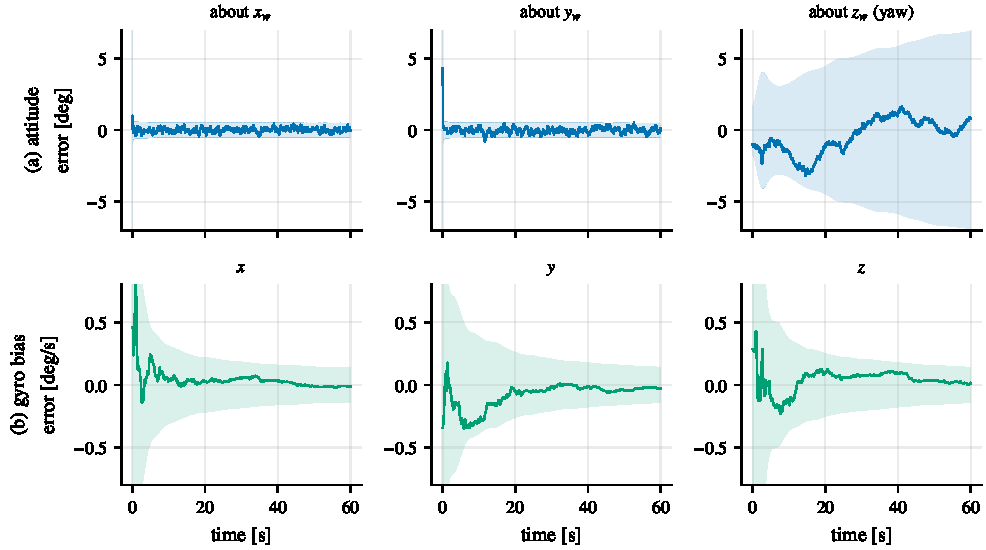
\includegraphics[width=\textwidth]{fig_ahrs.pdf}
  \caption{The attitude ESKF of \cref{sec:ahrs} on a simulated tumbling device: gyroscope at 100~Hz with a constant bias, accelerometer used as an
  inclinometer at 10~Hz. (a) Attitude errors about the world axes with their $\pm3\sigma$ bounds. Tilt (about $x$ and $y$) is quickly bounded by the
  accelerometer; the error about the vertical (yaw) is unobservable, and its bound grows. (b) Gyro bias errors with $\pm3\sigma$ bounds. The bias
  is never measured directly, yet all three components converge, because the device's rotation makes each body axis horizontal at some time.}
  \label{fig:ahrs}
\end{figure}

\Cref{fig:ahrs} shows the filter on simulated data. Several lessons of this chapter are visible in it. The errors stay inside their $3\sigma$
bounds: the filter is consistent. Tilt becomes accurate within seconds, through the accelerometer. Yaw is unobservable without a magnetometer
or vision, so its uncertainty only grows. And the gyro bias, although never measured, is estimated through its correlation with the tilt error
it causes: the cross-covariance built by propagation lets the gain correct it. This is exactly how the full VIO filter estimates IMU biases from
camera measurements.

\begin{projectlink}[Milestones 4--6]
M4 implements step 2 of \cref{alg:eskf}, M5 steps 3--4, and M6 the update, injection and reset with a pose measurement. Testing them separately
localizes bugs: if propagation is exact on synthetic data, and the covariance matches Monte Carlo statistics, then any later inconsistency is in
the update.
\end{projectlink}

\begin{takeaways}
\begin{itemize}
  \item The ESKF splits the state into a nonlinear nominal part and a small, minimal, nearly linear error part. The Kalman filter only ever sees the
        error.
  \item The error mean is zero during propagation; only $P$ is propagated.
  \item Residual $r = z\bminus h(\hat x) \approx H\delta x + n$ with $H$ the manifold Jacobian of $h$ at $\hat x$.
  \item After injection, reset $P \gets GPG\T$ with $G_\theta = I - \tfrac12\sx{\delta\hat\theta}$ for every (local) attitude block.
  \item The attitude example shows observability at work: gravity bounds tilt, yaw drifts, and unmeasured biases are estimated through
        correlations.
\end{itemize}
\end{takeaways}

\begin{exercises}
  \item Derive the reset Jacobian for the global perturbation $R = \Exp(\delta\theta)\hat R$ and confirm $G_\theta = I + \tfrac12\sx{\delta\hat\theta}$.
  \item Suppose $\delta\hat\theta = (0, 0, 0.1)$~rad and $P_{\theta\theta} = \diag(10^{-4}, 10^{-4}, 10^{-2})$. Compute $GP_{\theta\theta}G\T$ and compare with
        $\Jr(\delta\hat\theta)P_{\theta\theta}\Jr(\delta\hat\theta)\T$. When is the difference noticeable?
  \item An iterated ESKF repeats the update with $H$ re-evaluated at $\hat x\bplus\delta\hat x$. Show that one iteration is a Gauss--Newton step on the MAP cost
        $\|\delta x\|^2_{P\inv} + \|z\bminus h(\hat x\bplus\delta x)\|^2_{R_z\inv}$.
  \item Implement the attitude filter of \cref{sec:ahrs} and reproduce \cref{fig:ahrs}. Then hold the device still and observe which bias component stops
        converging. Explain why.
  \item Rewrite the attitude filter with the local perturbation $R = \hat R\Exp(\delta\theta)$: derive $F_c$, $G_c$, $H$ and $G$. (This is a small version of the project's
        derivation exercise.)
\end{exercises}
% Solutions to the exercises of Chapter 14.
\begin{solutions}
  \item With the global perturbation the true attitude is $R = \Exp(\delta\theta)\hat R$ before injection and $R = \Exp(\delta\theta^+)\hat R^+$ after it, with
        $\hat R^+ = \Exp(\delta\hat\theta)\hat R$. Equating, $\Exp(\delta\theta^+) = \Exp(\delta\theta)\Exp(-\delta\hat\theta)$, and the BCH formula \eqref{eq:bch} gives
        \[
          \delta\theta^+ = \delta\theta - \delta\hat\theta - \tfrac12\,\delta\theta\times\delta\hat\theta + \cdots = \delta\theta - \delta\hat\theta + \tfrac12\,\delta\hat\theta\times\delta\theta + \cdots,
        \]
        whose derivative with respect to $\delta\theta$ is $G_\theta = I + \tfrac12\sx{\delta\hat\theta}$. The sign is opposite to the local case
        (\cref{prop:reset}), because the correction now multiplies on the left. (Exactly, the derivative at $\delta\theta = \delta\hat\theta$ is $\Jl(\delta\hat\theta)$.)

  \item Here $\sx{\delta\hat\theta}$ mixes only $x$ and $y$, and $P_{\theta\theta}$ is isotropic in that plane, so both products stay diagonal:
        \begin{align*}
          GP_{\theta\theta}G\T &= \diag\big(1.0025,\ 1.0025,\ 100\big)\times10^{-4}, \\
          \Jr P_{\theta\theta}\Jr\T &= \diag\big(0.9992,\ 0.9992,\ 100\big)\times10^{-4}.
        \end{align*}
        The difference, $0.33\%$ of the $x$ and $y$ variances, is second order: $G$ and $\Jr(\delta\hat\theta) = I - \tfrac12\sx{\delta\hat\theta} + O(\|\delta\hat\theta\|^2)$ agree to
        first order, and their products differ by about $\|\delta\hat\theta\|^2/3$. For anisotropic covariances the first-order rotation of the covariance is the
        same in both, and the relative difference is about $3\times10^{-6}$, $3\times10^{-4}$, $3\%$ and $40\%$ for corrections of $0.003$, $0.03$, $0.3$ and $1$~rad. It
        is negligible for the milliradian corrections of a running filter and noticeable only after very large corrections, such as the first updates
        after a poor initialization.

  \item Let $\delta x$ be the error-state variable with prior $\N(0, P)$ in the tangent space at $\hat x$, and $r(\delta x) = z\bminus h(\hat x\bplus\delta x)$, so that the MAP
        cost is $F(\delta x) = \|\delta x\|^2_{P\inv} + \|r(\delta x)\|^2_{R_z\inv}$. Near an iterate $\delta x_i$, $r(\delta x) \approx r_i - H_i(\delta x - \delta x_i)$ with $r_i = r(\delta x_i)$ and $H_i$ the
        manifold Jacobian of $h$ at $\hat x\bplus\delta x_i$. Minimizing the resulting quadratic gives the Gauss--Newton iterate (the algebra of Exercise 10.7 with
        $\mu = 0$)
        \[
          \delta x_{i+1} = K_i\big(r_i + H_i\,\delta x_i\big), \qquad K_i = PH_i\T\big(H_iPH_i\T + R_z\big)\inv .
        \]
        From $\delta x_0 = 0$ the first iterate is $\delta x_1 = K_0r(0)$ with $H_0$ evaluated at $\hat x$: exactly the ESKF update $\delta\hat x = Kr$. One ESKF update is
        therefore one Gauss--Newton step on the MAP cost; the iterated ESKF re-evaluates $h$ and $H$ at $\hat x\bplus\delta x_i$ and repeats, then injects the final
        $\delta x$ and resets once.

  \item The code of \cref{fig:ahrs} is \code{fig\_ahrs} in \code{scripts/figures\_extra.py}. With the tumbling motion all three bias errors converge,
        ending with standard deviations of about $8\times10^{-4}$~rad/s and errors within them. Holding the device still and level (zero rate) instead, the
        two horizontal components still converge ($\sigma \approx 6.5\times10^{-4}$~rad/s, errors consistent with it), but the vertical component, along the measured
        gravity, does not: its error stays near its initial $0.01$~rad/s. A bias about the vertical integrates into a yaw error, and an inclinometer
        cannot see yaw; to first order that bias is unobservable. Under rotation, every body axis is horizontal at some time, and a bias about a
        horizontal axis produces a tilt that the accelerometer does see. (The filter's own $\sigma$ for the vertical component nevertheless shrinks to about
        $0.004$~rad/s, so its error sits near $2.7\sigma$. With the bias unobservable the yaw estimate drifts far from the truth, $0.3$~rad in a minute, and
        Jacobians evaluated at that drifting estimate inject information the data do not contain. Evaluated at the true attitude, the same filter's
        error is consistent with its $\sigma$. This is a first encounter with the mechanism analyzed in \cref{ch:observability}.)

  \item \ifsolutions
        With $R = \hat R\Exp(\delta\theta)$, $\hat\omega = \omega_m - \hat b$ and $\omega = \omega_m - b - n_g = \hat\omega - \delta b - n_g$, \cref{lem:dexp} applied to
        $\dot R = R\sx{\omega}$ gives, to first order, $\dot{\delta\theta} = -\sx{\hat\omega}\delta\theta - \delta b - n_g$; and $\dot{\delta b} = n_b$. Hence
        \[
          F_c = \begin{bmatrix}-\sx{\hat\omega} & -I\\ 0 & 0\end{bmatrix}, \qquad G_c = \begin{bmatrix}-I & 0\\ 0 & I\end{bmatrix}.
        \]
        For the inclinometer, $h = R\T v$, and the inverse-action row of \cref{tab:jacobians} gives
        \[
          h(\hat R\Exp(\delta\theta)) \approx \hat R\T v + \sx{\hat R\T v}\,\delta\theta, \qquad\text{so}\qquad H = \big[\sx{\hat R\T v}\ \ 0\big].
        \] The reset is $G = \blkdiag\big(I - \tfrac12\sx{\delta\hat\theta},\ I\big)$ (\cref{prop:reset}). Compared with the global version of
        \cref{sec:ahrs}, the heading-dependent $\hat R$ has disappeared from $F_c$ and $G_c$ and moved into $H$, and the error is coupled to the rotation through
        $-\sx{\hat\omega}$: a body-frame error appears to rotate backwards as the body turns. These are exactly the attitude rows of the project's $F_c$ and $G_c$.
        \else\withheldsolution\fi
\end{solutions}

